
\documentclass{article}
\usepackage[paperwidth=90mm, paperheight=50mm, margin=5mm]{geometry}
\usepackage{tikz}
\usepackage{graphicx}
\usepackage{fontawesome5}
\pagestyle{empty}
\usetikzlibrary{positioning}

\begin{document}
\begin{tikzpicture}[remember picture, overlay]
    % Light blue background
    \fill[blue!5] (current bounding box.south west) rectangle (current bounding box.north east);

    % Aircraft shape in top-right corner
    \begin{scope}[shift={(7.2,4)}]
        \draw[thick, blue!70!black] (0,0) -- (0.4,0.2) -- (0.4,-0.2) -- cycle; % fuselage
        \draw[thick, blue!70!black] (0,0) -- (-0.3,0.15); % left wing
        \draw[thick, blue!70!black] (0,0) -- (-0.3,-0.15); % right wing
    \end{scope}

    % Name and title
    \node[anchor=west, text=blue!80!black] at (0,3.2) {\textbf{\Large Amaury Bilocq}};
    \node[anchor=west] at (0,2.7) {Aerospace \& Industrial Engineer};
    \node[anchor=west] at (0,2.3) {PhD in Numerical Methods};

    % Contact info
    \node[anchor=west] at (0,1.6) {\faEnvelope\ \ amaury.bilocq@gmail.com};
    \node[anchor=west] at (0,1.2) {\faLinkedin\ \ linkedin.com/in/amaurybilocq};
    \node[anchor=west] at (0,0.8) {\faMapMarker*\ \ Liège, Belgium};

    % QR code on right
    \node[anchor=north east] at (8,2.5) {
        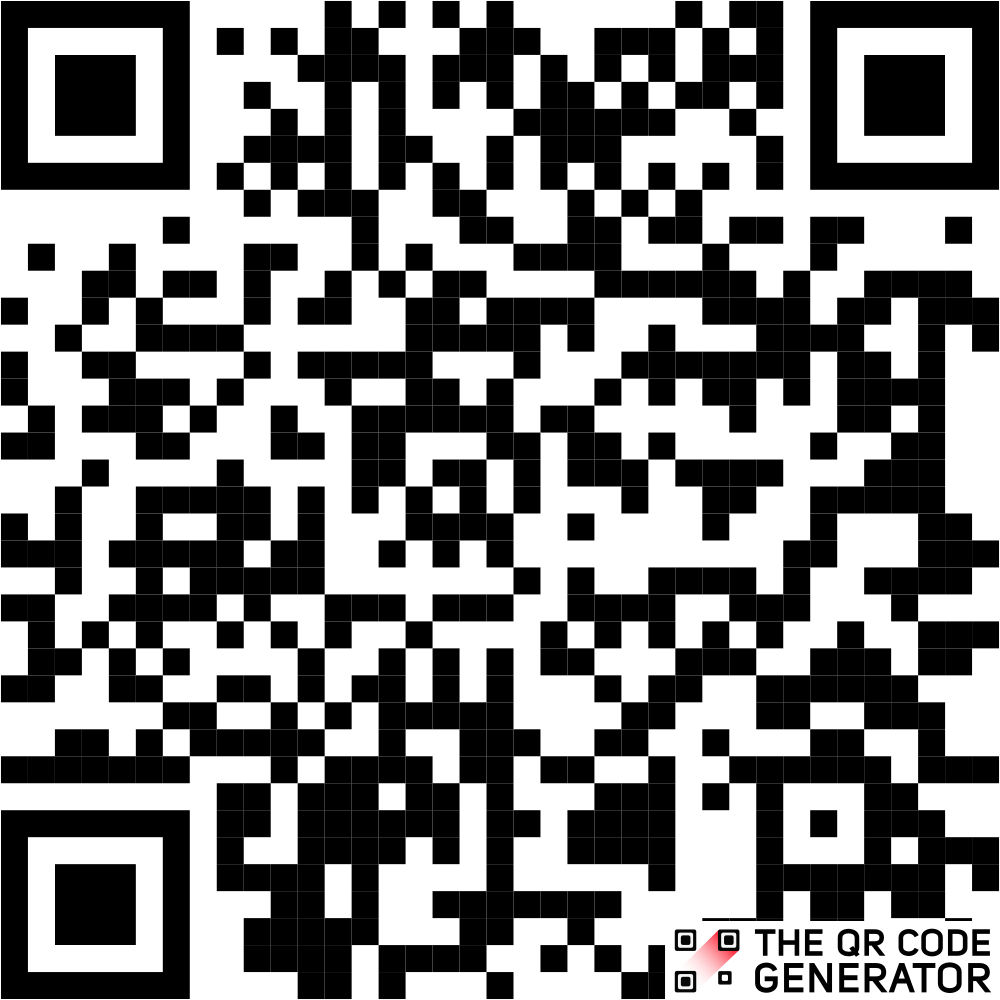
\includegraphics[width=2.5cm]{cvABilocq.png}
    };
\end{tikzpicture}
\end{document}
